% ****** Start of file apssamp.tex ******
%
%   This file is part of the APS files in the REVTeX 4.2 distribution.
%   Version 4.2a of REVTeX, December 2014
%
%   Copyright (c) 2014 The American Physical Society.
%
%   See the REVTeX 4 README file for restrictions and more information.
%
% TeX'ing this file requires that you have AMS-LaTeX 2.0 installed
% as well as the rest of the prerequisites for REVTeX 4.2
%
% See the REVTeX 4 README file
% It also requires running BibTeX. The commands are as follows:
%
%  1)  latex apssamp.tex
%  2)  bibtex apssamp
%  3)  latex apssamp.tex
%  4)  latex apssamp.tex
%
\documentclass[%
reprint,
%superscriptaddress,
%groupedaddress,
%unsortedaddress,
%runinaddress,
%frontmatterverbose, 
%preprint,
%preprintnumbers,
%nofootinbib,
%nobibnotes,
%bibnotes,
amsmath,amssymb,
aps,
pra,
%prb,
%rmp,
%prstab,
%prstper,
%floatfix,
]{revtex4-2}

\usepackage{subfiles}
\usepackage{graphicx}% Include figure files
\usepackage{dcolumn}% Align table columns on decimal point
\usepackage{bm}% bold math
\usepackage{float}
\usepackage{mathtools}
\usepackage{xcolor}
\usepackage{physics}
\usepackage{dsfont}
\usepackage{tcolorbox}
\usepackage{float}
\usepackage{tensor}
\usepackage{hyperref}% add hypertext capabilities
%\usepackage[mathlines]{lineno}% Enable numbering of text and display math
%\linenumbers\relax % Commence numbering lines

%\usepackage[showframe,%Uncomment any one of the following lines to test 
%%scale=0.7, marginratio={1:1, 2:3}, ignoreall,% default settings
%%text={7in,10in},centering,
%%margin=1.5in,
%%total={6.5in,8.75in}, top=1.2in, left=0.9in, includefoot,
%%height=10in,a5paper,hmargin={3cm,0.8in},
%]{geometry}
\newcommand{\Hp}{\mathcal{H}}
\renewcommand{\thesection}{\arabic{section}}
\renewcommand{\thesubsection}{\thesection.\arabic{subsection}}
\renewcommand{\thesubsubsection}{\thesubsection.\arabic{subsubsection}}
\renewcommand{\figurename}{Fig.}
\renewcommand{\tablename}{Table}
\makeatletter
\renewcommand{\subsubsection}{%
	\@startsection
	{subsubsection}%
	{3}%
	{\z@}%
	{.8cm \@plus1ex \@minus .2ex}%
	{.5cm}%
	{\normalfont\small\centering}%
}
\makeatother
\renewcommand{\L}{\mathcal{L}}
\renewcommand{\O}{\mathcal{O}}
\newcommand{\f}[2]{\frac{#1}{#2}}
\newcommand{\p}{\partial}

\begin{document}
	
\title{Project 1}
\author{Isak O. Rukan}
\email{Insert Email}
\author{Edvard B. Rørnes}
\email{e.b.rornes@fys.uio.no}
\affiliation{Institute of Physics, University of Oslo,\\0371 Oslo,  Norway}
\date{\today}

\begin{abstract}
	We investigate and compare three regression models\footnote{GitHub Repository: \url{https://github.com/EdvardRornes/FYS-STK4155/tree/main/Project1}}: Ordinary Least Squares, Ridge, and Least Absolute Shrinkage and Selection Operator. These were applied and analyzed on a two-dimensional Franke function and later tested on real terrain data from the US Geological Survey Earth Explorer \cite{USGS_EarthExplorer}. The models' performances are evaluated using metrics such as the Mean Squared Error and the coefficient of determination $R^2$. The bias-variance trade-off for OLS is studied in detail where it was found that ... (TBD). We used resampling techniques such as bootstrapping and cross-validation to probe the quality of the evaluations and determine the predictiveness and generalizability of the models. In our analysis the best performing method was ... (TBD).
\end{abstract}

\maketitle

\section{Introduction}
Regression models are essential tools in data analysis and prediction, particularly within the realm of physics. They are used to enable understanding of the relationships between different variables and improve our ability to create predictions. In this report we study and compare three common regression techniques: Ordinary Least Squares (OLS) regression, Ridge regression and Least Absolute Shrinkage and Selection Operator (LASSO) regression. Each come with their unique strengths and weaknesses that make them suitable for different data sets. 

OLS is the simplest and most foundational method which estimates relationship by minimizing the difference between observed and predicted values. A large downside with OLS is when there are many related variables as this can lead to unstable coefficient estimates \cite{Bishop2006}. Ridge regression can partially fix this issue by adding a penalty to large coefficients via a regulator $\lambda$, effectively allowing us to shrink the coefficients with a new input parameter. This in turn creates a more stable model in the event of correlated variables. LASSO regression takes this a step further by once again shrinking coefficients, but also setting some of them to zero. This allows LASSO to effectively choose important variables, which may be helpful when pursuing a simpler model.

To compare these regression model, we use a two-dimensional Franke function which allows us to test the performance of each under controlled conditions. Later we apply each model to real terrain data which is obtained from \cite{USGS_EarthExplorer}.

The models are evaluated by considering their Mean Squared Error (MSE) and coefficient of determination $R^2$. Further to make our evaluation more reliable, resampling techniques such as bootstrapping and cross-validation are used. These methods provide a quantatitive description of how well each model performs on different data sets.
\section{Theory}
All claims made in this section which require relatively lengthy derivations are derived in Appendix \ref{Appendix:Derivations}. The general structure of all our models is that we have some data set $\{x_i,y_i\}$ where $i\in\{0,1...,n-1\}$ where $x_i$ are independent variables whilst $y_i$ are dependent variables. The data is assumed to be described by
\begin{align}
	\bm y=f(\bm x)+\bm \varepsilon
	\label{eq:data}
\end{align}
where $f$ is some continuous function which takes $\bm x$ as input and $\bm\varepsilon$ is a normal distributed error $\bm\varepsilon\sim\mathcal{N}(0,\sigma^2)$. The function $f$ will then be approximated with a model $\tilde{\bm y}$ in which we will consider a polynomial expansion with coefficients $\beta_i$:
\begin{align}
	\tilde{y}_i=\sum_{j=0}^{p-1}\beta_j x_i^j
	\label{eq:model}
\end{align}
defining the $n\times p$ design matrix $\bm X$ with elements $X_{ij}=(x_i)^j$ we can rewrite this as
\begin{align}
	\tilde{\bm y}=\bm X\bm\beta
\end{align}
Further, each model will be defined with a different cost function $C(\bm\beta)$ which we minimize to find the coefficients for each respective model.

The metrics MSE and $R^2$ which we use to analyze each model are defined by
\begin{align}
	\text{MSE}(\bm y,\tilde{\bm{y}})&\equiv\frac{1}{n}\sum_{i=0}^{n-1}(y_i-\tilde y_i)^2,\\
	R^2&\equiv1-\frac{\sum_{i=0}^{n-1}(y_i-\tilde y_i)^2}{\sum_{i=0}^{n-1}(y_i-\bar y)^2}
\end{align}
where $\bar y\equiv\frac{1}{n}\sum_{i=0}^{n-1}y_i$ is the mean value of $\bm y$. Here we can see that if $\tilde{\bm{y}}=\bm y$ then $R^2=1$ implies that we have perfect accuracy. Further if $\tilde{\bm{y}}$ is simply the mean then $R^2=0$ implying that our fit is equally bad as a single line and if $R^2<0$ it means that our approximation is worse than simply taking the mean.

\subsection{OLS}
OLS is a primitive method used in linear regression to estimate coefficients of a linear model. The cost function in OLS is simply defined as the residual sum of squares (RSS)
\begin{align*}
	C_\text{OLS}(\bm\beta)=\text{RSS}(\bm\beta)=(\bm y-\tilde{\bm y})^2=(y_i-X_{ij}\beta_j)^2
\end{align*}
where we employ the summation notation where repeated indices are summed over. As mentioned prior, the coefficients $\bm\beta$ are found by minimizing the cost function, i.e. taking the derivative w.r.t. $\bm\beta$. This results in
\begin{align*}
	\bm\beta_\text{OLS}=(\bm X^T\bm X)^{-1}\bm X^T\bm y
\end{align*}
which yields the model
\begin{align}
	\tilde{\bm y}_\text{OLS}=\bm X\bm \beta_\text{OLS}
\end{align}
Assuming our data takes the form of (\ref{eq:data}) then the expectation value $\bm y$ is
\begin{align*}
	\mathbb{E}(y_i)=\mathbb{E}(f(x_i))=X_{ij}\beta_j\equiv\bm X_{i,*}\bm\beta
\end{align*}
since $\mathbb{E}(\varepsilon_i)=0$ follows from its definition. The variance of $\bm y$ is given by
\begin{align*}
	\text{Var}(y_i)=\text{Var}(\varepsilon_i^2)=\sigma^2
\end{align*}
which yields $y_i\sim\mathcal{N}(\bm X_{i,*}\bm\beta,\sigma^2)$. The expectation value of the optimal parameters $\hat{\bm\beta}$ can be found to be
\begin{align*}
	\mathbb{E}(\hat{\bm\beta}_\text{OLS})=\bm\beta.
\end{align*}
with the variance
\begin{align*}
	\text{Var}(\hat{\bm\beta}_\text{OLS})=\sigma^2(\bm X^T \bm X)^{-1}
\end{align*}

\subsection{Ridge}
Ridge regression is an extension of OLS where define the cost function as a modified version of the OLS cost function with an added penalty term which is proportional to the coefficients $\beta_i^2$:
\begin{align}
	C_\text{Ridge}(\bm\beta)=C_\text{OLS}(\bm\beta)+\lambda\bm\beta^2
	\label{eq:cost_ridge}
\end{align}
Here $\lambda\geq0$ is a regularization parameter, or commonly referred to as a hyperparameter, which controls the strength of this additional penalty. This regulator essentially drives the magnitude of these coefficients allowing for more tweaking in the parameter space. This parametrization of course includes the constraint that $\bm{\beta}^2\leq t$ for some $t<\infty$ such that we can choose our arbitrary parameter $\lambda\geq0$ to be sufficiently small s.t. the cost function (\ref{eq:cost_ridge}) does not diverge. The optimal parameters for Ridge regressions can again be found by the same process as for OLS:
\begin{align*}
	\bm{\beta}&=(\bm{X}^T\bm{X}+\lambda\bm{I})^{-1}\bm{X}^T\bm{y}
\end{align*}
Here we can see that the effect of adding this penalty term is essentially taking $(\bm X^T\bm X)^{-1}\to(\bm X^T\bm X+\lambda\bm I)^{-1}$ when compared to the OLS case. In the past this was generally the starting point for Ridge regression in the cases where the matrix $\bm X^T\bm X$ was not invertible. A direct way of seeing the effect of the regulator is by considering the singular value decomposition (SVD) of $\bm X$. Doing so one can show that 
\begin{align}
	\tilde{\bm{y}}_\text{Ridge}=\sum_{j=0}^{p-1}\bm{u}_j\bm{u}_j^T\frac{\sigma_j^2}{\sigma_j^2+\lambda}\bm{y}
	\label{eq:beta_ridge}
\end{align}
where $\bm u_i$ is the $i$-th row (column?) of the orthogonal matrix $\bm U$ stemming from the SVD: $\bm X=\bm U\bm \Sigma\bm V$. Since $\lambda\geq0$ then this added factor compared to OSL is $\leq1$. We can then see that Ridge regression effectively suppresses all the coefficients, thus $\lambda$ is often called the "shrinkage" factor. 

\subsection{LASSO}
Similarly to Ridge, LASSO also includes a penalty factor. The cost function in this case is instead defined to be
\begin{align}
	C_\text{LASSO}(\bm\beta)=C_\text{OLS}(\bm\beta)+\lambda||\bm\beta||_1
	\label{eq:cost_lasso}
\end{align}
where
\begin{align*}
	||\bm\beta||_k\equiv\left[\sum_{i=0}^{n-1}|\beta_i|^k\right]^{1/k}
\end{align*}
is the $L^k$ norm of $\bm\beta$. Taking the derivative of (\ref{eq:cost_ridge}) w.r.t. $\bm \beta$ and requiring that this becomes zero we have
\begin{align}
	0=\pdv{C_\text{LASSO}}{\bm\beta}=-2\bm X^T(\bm y-\bm X\bm\beta)+\lambda\,\text{sgn}(\bm\beta)
\end{align}
This has the added benefit of being able to set certain parameters to be $0$ instead of suppressing them, at the cost of losing analytical expressions for $\hat{\bm\beta}$ in non-trivial cases.

\subsection{Connection to Statistics}
The three aforementioned regression techniques all have relatively simple connections to statistical probability distribution functions. Assuming that the likelihood of an event $y_i$ with the input variables $\bm X$ and parameters $\bm\beta$ is given by a Gaussian distribution:
\begin{align}
	p(y_i,\bm X|\bm\beta)=\prod_{i=0}^{n-1}\frac{1}{\sqrt{2\pi\sigma^2}}\exp\left[-\frac{(y_i-\bm X_{i,*}\bm\beta)^2}{2\sigma^2}\right]
\end{align}
Further assuming that all events are independent and identically distributed the total probability density function takes the form
\begin{align}
	p(\bm y,\bm X|\bm\beta)=\prod_{i=0}^{n-1}p(y_i,\bm X|\bm\beta)
\end{align}
then taking the negative logarithm of the above and defining that as our cost function we can arrive at the exact expression for the cost function that we defined earlier, i.e. just the RSS which corresponds to OLS. A similar analysis for Ridge can be done. Using Bayes' theorem we have that $p(\bm\beta|\bm X,\bm y)\propto p(\bm y,\bm X|\bm\beta)p(\bm\beta)$ we then feed in the prior:
\begin{align}
	p(\beta_i)=\exp\left[-\frac{\beta_i^2}{2\tau^2}\right]
\end{align}
one arrives at the probability of the coefficients $\bm\beta$ given the data $\bm y$
\begin{align}
	p(\bm\beta|\bm X,\bm y)\propto p(\bm y,\bm X|\bm\beta)\cdot\prod_{i=0}^{p-1}\exp\left[-\frac{\beta_i^2}{2\tau^2}\right]
\end{align}
Again, defining the cost function as the negative logarithm of this expression one arrives at the Ridge cost function with $\lambda=1/(2\tau^2)$. Finally for LASSO one assumes that the initial probability is given by the same as OLS but with the addition of the $\beta$ coefficients following a Laplace distribution
\begin{align}
	p(\beta_i)=\exp\left[-\frac{|\beta_i|}{\tau}\right]
\end{align}
one arrives at the LASSO cost function with $\lambda=1/\tau$. These statistical connections help us better understand the assumptions made with each technique. With OLS one assumes that each event $y_i$ are all independent and Gaussian. Thus when this is not the case one should not be surprised if OLS performs poorly. Ridge and LASSO however do account for the chance that there are correlated events, and assumes that the coefficients that we compute are themselves Gaussian or Laplace distributed. The hyperparameter $\lambda$ now has a clear interpretation, i.e. that we essentially insert a standard deviation of the $\beta$ coefficients. The performance of these latter two can then also be used to indicate which distribution more accurately describes the coefficients.

\subsection{Bias-Variance}
The so-called Bias-Variance Trade-Off can be summarized in a single equation:
\begin{align}
	\mathbb{E}[(\bm y-\tilde{\bm y})^2]=\text{Bias}[\tilde{\bm y}]+\text{Var}[\tilde{\bm y}]+\sigma^2
	\label{eq:MSE-bias-var}
\end{align}
The LHS of (\ref{eq:MSE-bias-var}) is the expected value of the MSE which tells us how well the model's predictions match the true data on average. The equation shows that we can decompose this expected MSE into 3 different components.
\begin{itemize}
	\item Bias: This quantity measures how much the model's average prediction differs from its true value. A high bias implies that the model is underfitting the data of is simply too simplistic.
	\item Var: The variance measures how much the model's predictions vary when trained on different datasets. It captures the sensitivity of the model to small changes in the training data. A high variance suggests overfitting, meaning it performs well on the training data but may be capturing noise or false patterns.
	\item $\sigma^2$: This is the irreducible error or noise in the data itself which cannot be explained by the model.
\end{itemize}
The idea is to minimize the LHS of (\ref{eq:MSE-bias-var}), so clearly we want to minimize both the bias and the variance at the same time. However these are correlated to one another, so lowering the e.g. the bias will in general increase the variance. So Bias-Variance Tradeoff is essentially trying to optimize the complexity of the model such that we neither overfit nor underfit the model such that it can be generalized to other cases. These quantities can then be used as means to fine tune a model.

\subsection{Resampling}
Resampling techniques are critical in understanding the performance and robustness of a model. They tend to better show how well a model will do on data it has not seen before, and are thus useful for diagnosing problems like over- and underfitting. In this report focus on two resampling methods: bootstrapping and cross-validation.

\subsubsection{Bootstrap} 
Bootstrapping is a statistical method that involves taking random samples with replacement from the original dataset to create several new datasets. These datasets are the same size as the original dataset, but since our sampling was done with replacement, some observations are presented more than once whilst others are eliminated. Here we train and evaluate a model over each of these resampled datasets, allowing us to estimate how the performance varies across different datasets. This method is particularly important when the datasets are small as it heavily increases the amount information that can be extracted from a given data set. Averaging across all the performance metrics from these little bootstrap samples provides a much more robust description of how well our model performs. 

\subsubsection{Cross-Validation} 
$k$-fold cross-validation is the other resampling method which we considered in this project. In $k$-fold cross-validation, the dataset is divided into $k$ subsets (or folds). The model is trained on $k-1$ of these folds and tested on the remaining fold. This process is repeated $k$ times, with each fold serving as the test set exactly once. The performance metrics, MSE and $R^2$, are averaged over the $k$ iterations to provide a more reliable estimate of how the model performs on unseen data.

Cross-validation is particularly advantageous for its ability to reduce the variance of performance estimates by using different portions of the data for both training and validation. In our analysis, we used 5-fold cross-validation to evaluate the stability and predictive power of each regression method. This method gave us a clearer picture of how each model generalizes, helping us tune the hyperparameters, such as the regularization parameter $\lambda$ for Ridge and LASSO.

Both resampling techniques are used to gain valuable insights into model performance and ensure that the conclusions drawn from our analysis are not overly dependent on a particular division of the dataset.

\section{Implementation}
For this project the surface we will consider is given by the Franke function:
\begin{align}
	f(x,y)&=\frac{3}{4}\exp(-\frac{(9x-2)^2}{4}-\frac{(9y-2)^2}{4})\nonumber\\
	&+\frac{3}{4}\exp(-\frac{(9x+1)^2}{49}-\frac{(9y+1)^2}{10})\nonumber\\
	&+\frac{1}{2}\exp(-\frac{(9x-7)^2}{4}-\frac{(9y-3)^2}{4})\nonumber\\
	&-\frac{1}{5}\exp(-(9x-4)^2-(9y-7)^2)
\end{align}
This function maps a surface defined on the interval $x,y\in[0,1]$. To perform an analysis on this function we consider a polynomial fit up to degree $n$ analogous to (\ref{eq:model}) where:
\begin{align}
	\tilde{\bm{z}}&=\f1{n+1}\sum_{i=0}^{n}\bigg(\bm\beta_{0,0}\nonumber\\
	&+\bm\beta_{1,0}x_i+\bm\beta_{1,1}y_i\nonumber\\
	&+\bm\beta_{2,0}x_i^2+\bm\beta_{2,1}x_iy_i+\bm\beta_{2,2}y_i^2\nonumber\\
	&+...\nonumber\\
	&+\bm\beta_{n,0}x_i^n+\bm\beta_{n,1}x_i^{n-1}y+...+\bm\beta_{n,n-1}x_iy_i^{n-1}+\bm\beta_{n,n}y_i^n\bigg)\nonumber\\
	&=\frac{1}{n+1}\sum_{i,j=0}^{n}\sum_{\substack{k=0}}^{j}\bm\beta_{j,k} x^{j-k}_i y^{k}_i\equiv \bm X\bm\beta\label{eq:bmz}
\end{align}
Here the components $x_i$ and $y_i$ are entries in the input vectors $\bm x^T=\begin{bmatrix} x_0&...&x_n \end{bmatrix}$ and $\bm y^T=\begin{bmatrix} y_0& ...&y_n \end{bmatrix}$ respectively which are our independent variables. Each $\bm\beta_{i,j}$ is a $\frac{(n+1)(n+2)}{2}$ component vector with a single non-zero entry with magnitude $\beta_{i,j}$ and the design matrix $\bm X$ is then an $(n+1)\times\frac{(n+1)(n+2)}{2}$ matrix of the form:
\begin{align*}
	\bm X=\frac{1}{n+1}\begin{bmatrix}
		1 & x_0 & y_0 & x^2_0 & x_0y_0 & y_0^2 & ... & x_0^n & ... & y_0^n\\
		1 & x_1 & y_1 & x_1^2 & x_1y_1 & y_1^2 & ... & x_1^n & ... & y_1^n\\
		\vdots & \vdots & \vdots & \vdots & \vdots & \vdots & \ddots & \vdots & \ddots & \vdots\\
		1 & x_n & y_n & x_n^2 & x_ny_n & y_n^2 & ... & x_n^n & ... & y_n^n
	\end{bmatrix}
\end{align*}
and the $\bm\beta$ vector contains the $\frac{(n+1)(n+2)}{2}$ components 
\begin{align*}
	\bm\beta^T=\begin{bmatrix}
		\beta_{0,0}&\beta_{1,0}&\beta_{1,1}&\beta_{2,0}&\beta_{2,1}&\beta_{2,2}&...&\beta_{n(n-1)}&\beta_{n,n}
	\end{bmatrix}
\end{align*}
It should now be clear which unit vectors correspond to each term in (\ref{eq:bmz}).

We then generated data with the Franke function and used an $x$-$(1-x)$ train-test split. This was chosen because... For all the techniques we scaled our data because...

The OLS and Ridge regression fitting was done use of (\ref{eq:beta_ridge}) where for the prior we simply set $\lambda=0$. Since LASSO is more complicated we opted into using \texttt{sklearn.linear\_model}. Note that this excludes intercept by default so ... (?). The MSE and $R^2$ for all regression techniques were calculated with the \texttt{sklearn}'s \texttt{mean\_squared\_error} and \texttt{r2\_score} respectively. 


\section{Results}
\begin{figure}[ht!]
	\centering
	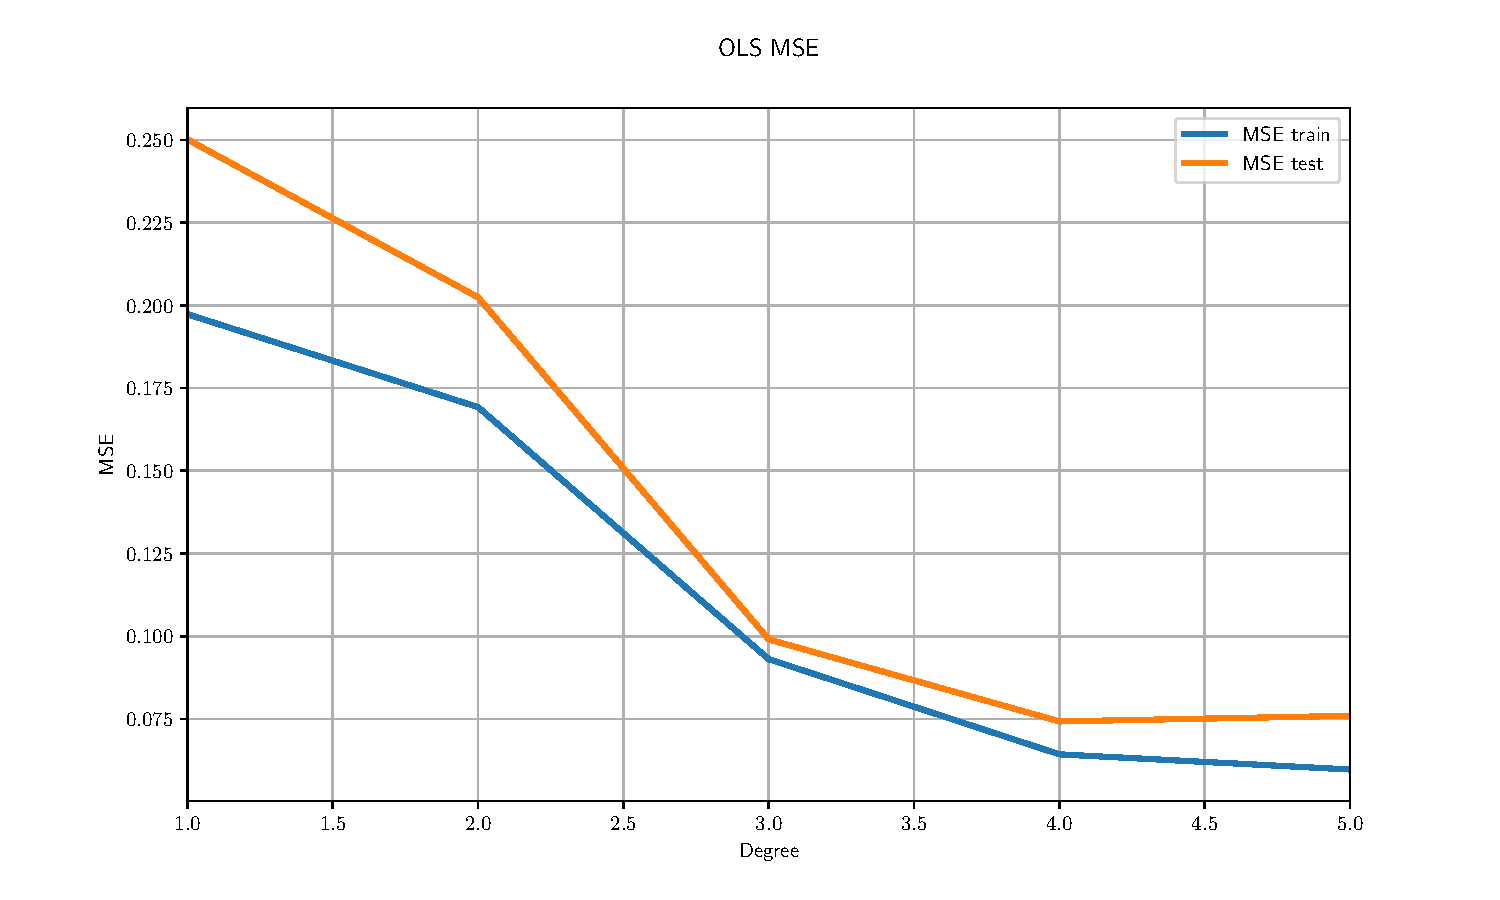
\includegraphics[width=\linewidth]{Python/Figures/OLS-MSE-degree.pdf}
	\caption{Caption}
	\label{fig:OLS_mse_degree}
\end{figure}
\begin{figure}[ht!]
	\centering
	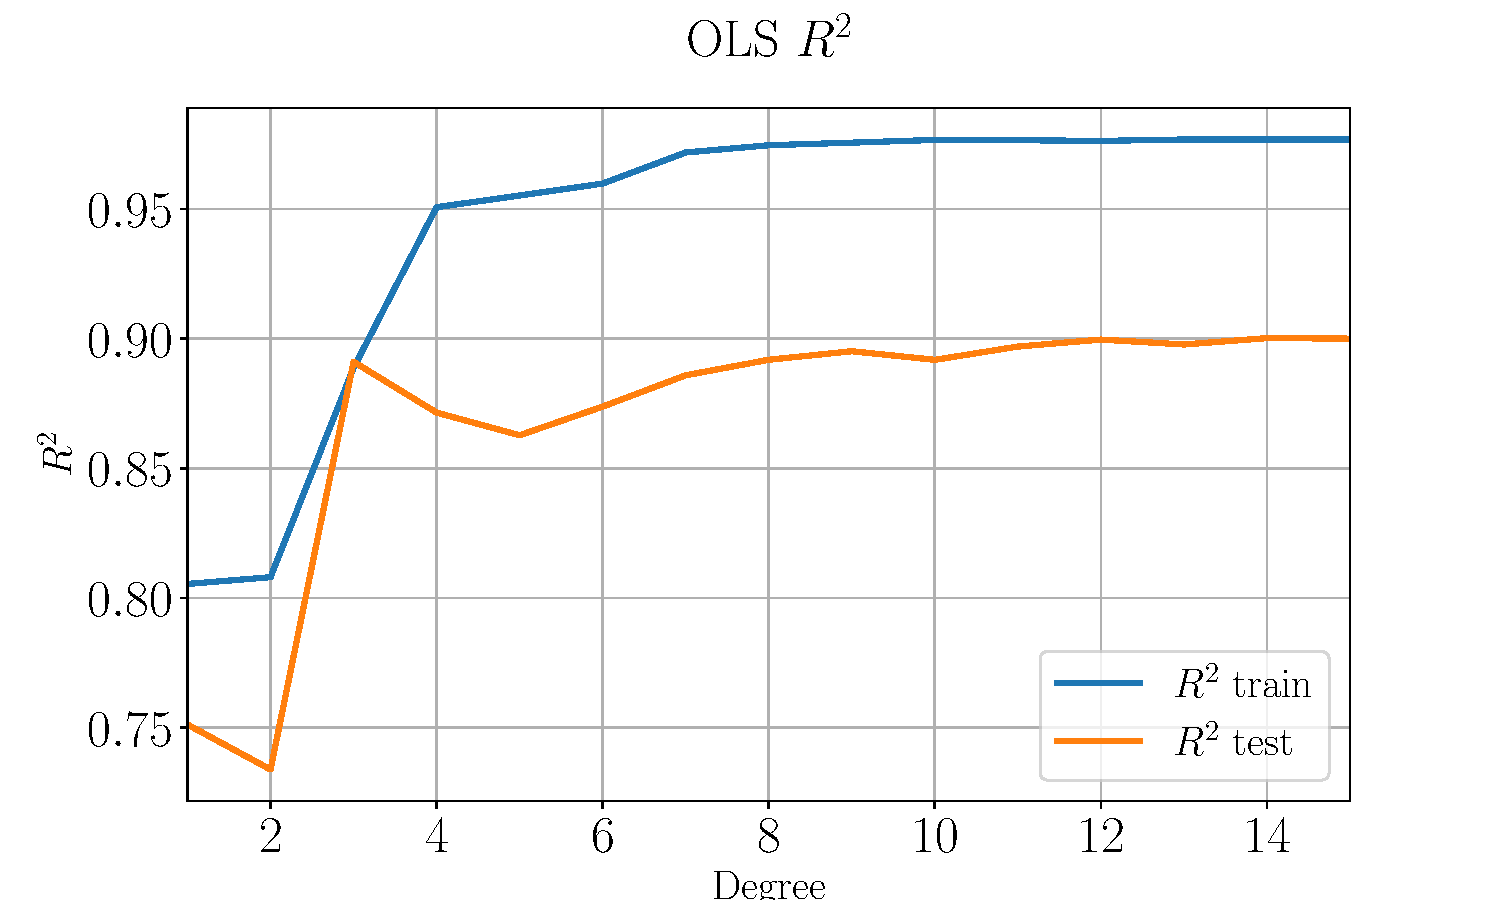
\includegraphics[width=\linewidth]{Python/Figures/OLS-R2-degree.pdf}
	\caption{Caption}
	\label{fig:OLS_r2_degree}
\end{figure}
\begin{figure}[ht!]
\centering
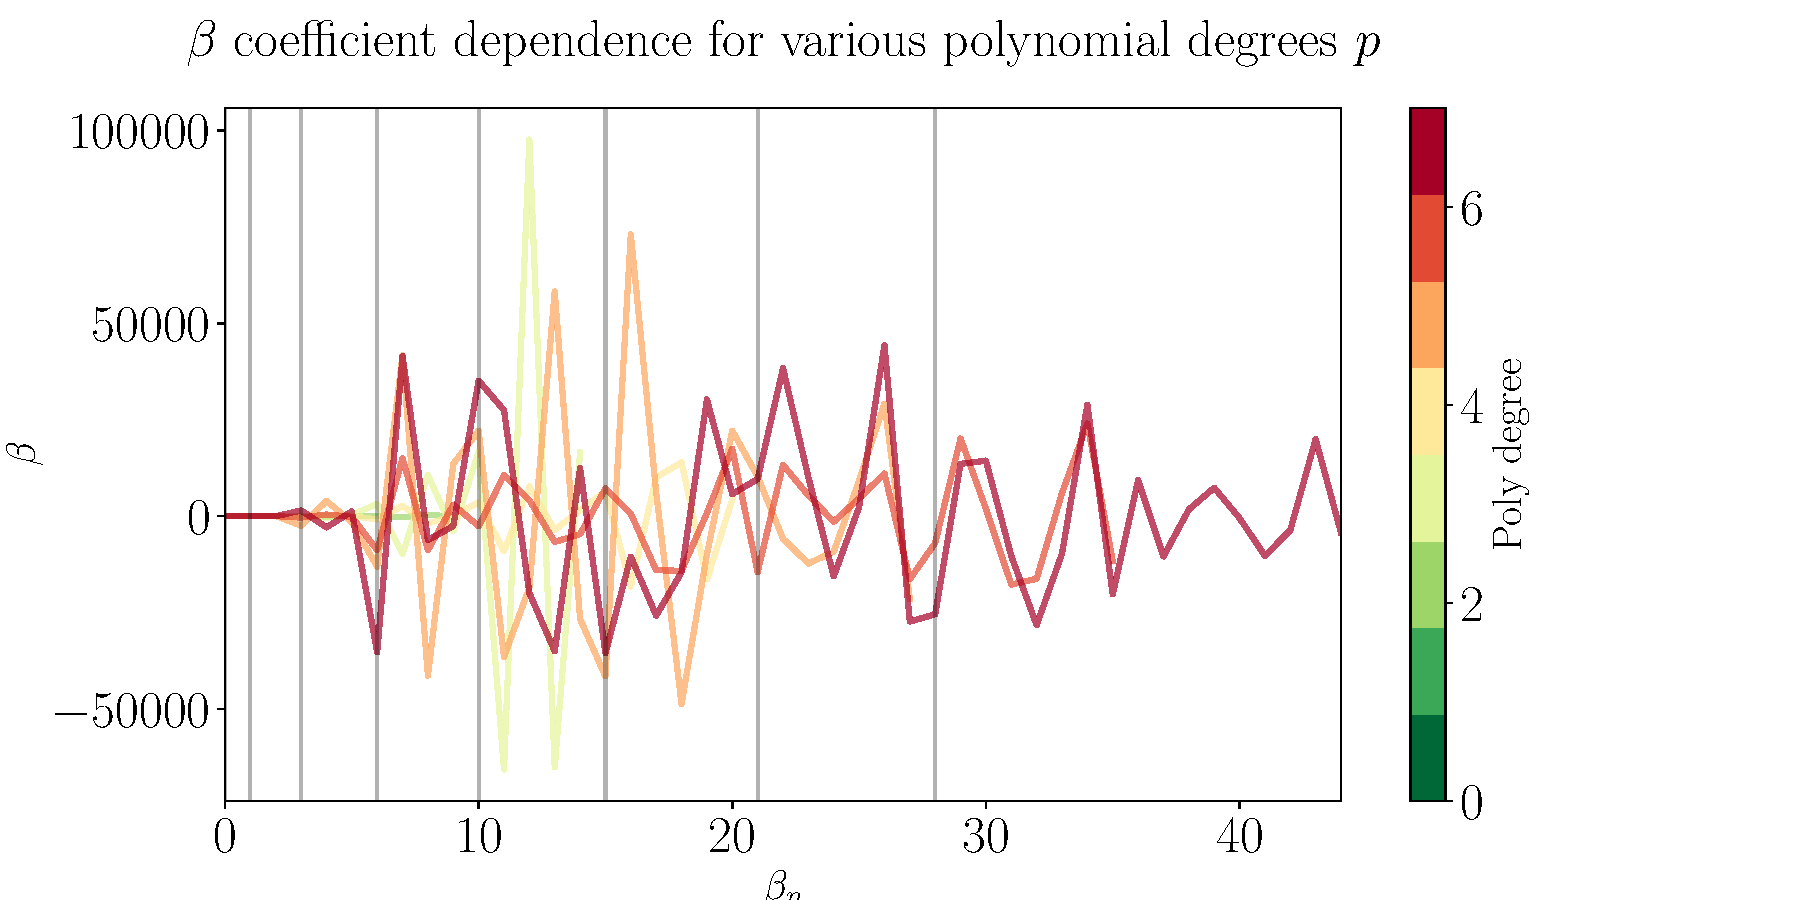
\includegraphics[width=\linewidth]{Python/Figures/OLS-beta-degree.pdf}
\caption{Caption}
\label{fig:OLS_beta_degree}
\end{figure}
\begin{figure}[ht!]
	\centering
	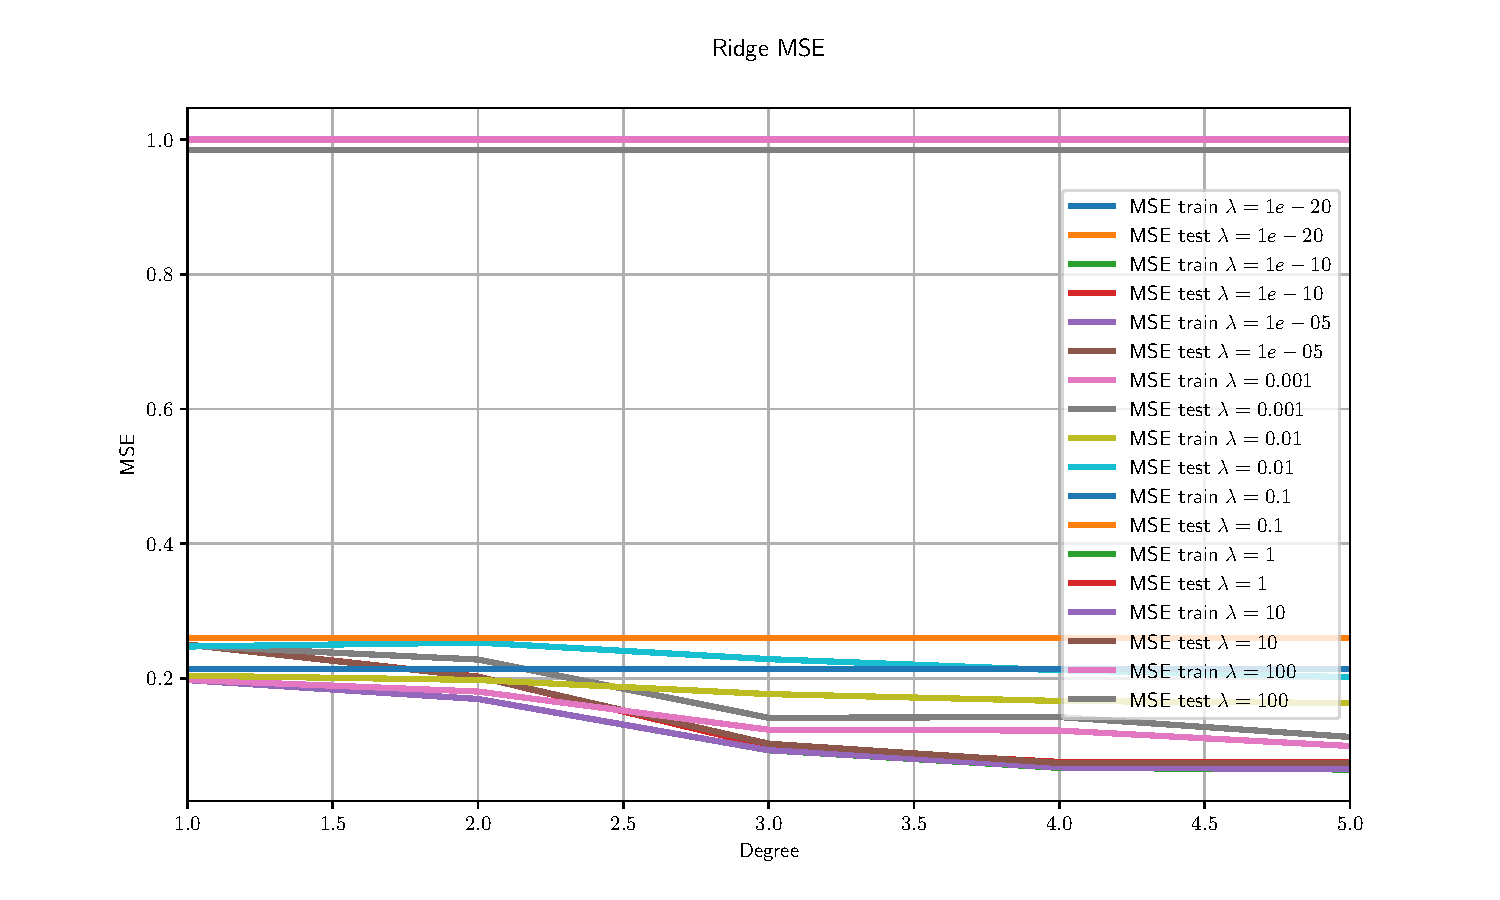
\includegraphics[width=\linewidth]{Python/Figures/Ridge-MSE-degree.pdf}
	\caption{Caption}
	\label{fig:ridge_mse_degree}
\end{figure}
\begin{figure}[ht!]
	\centering
	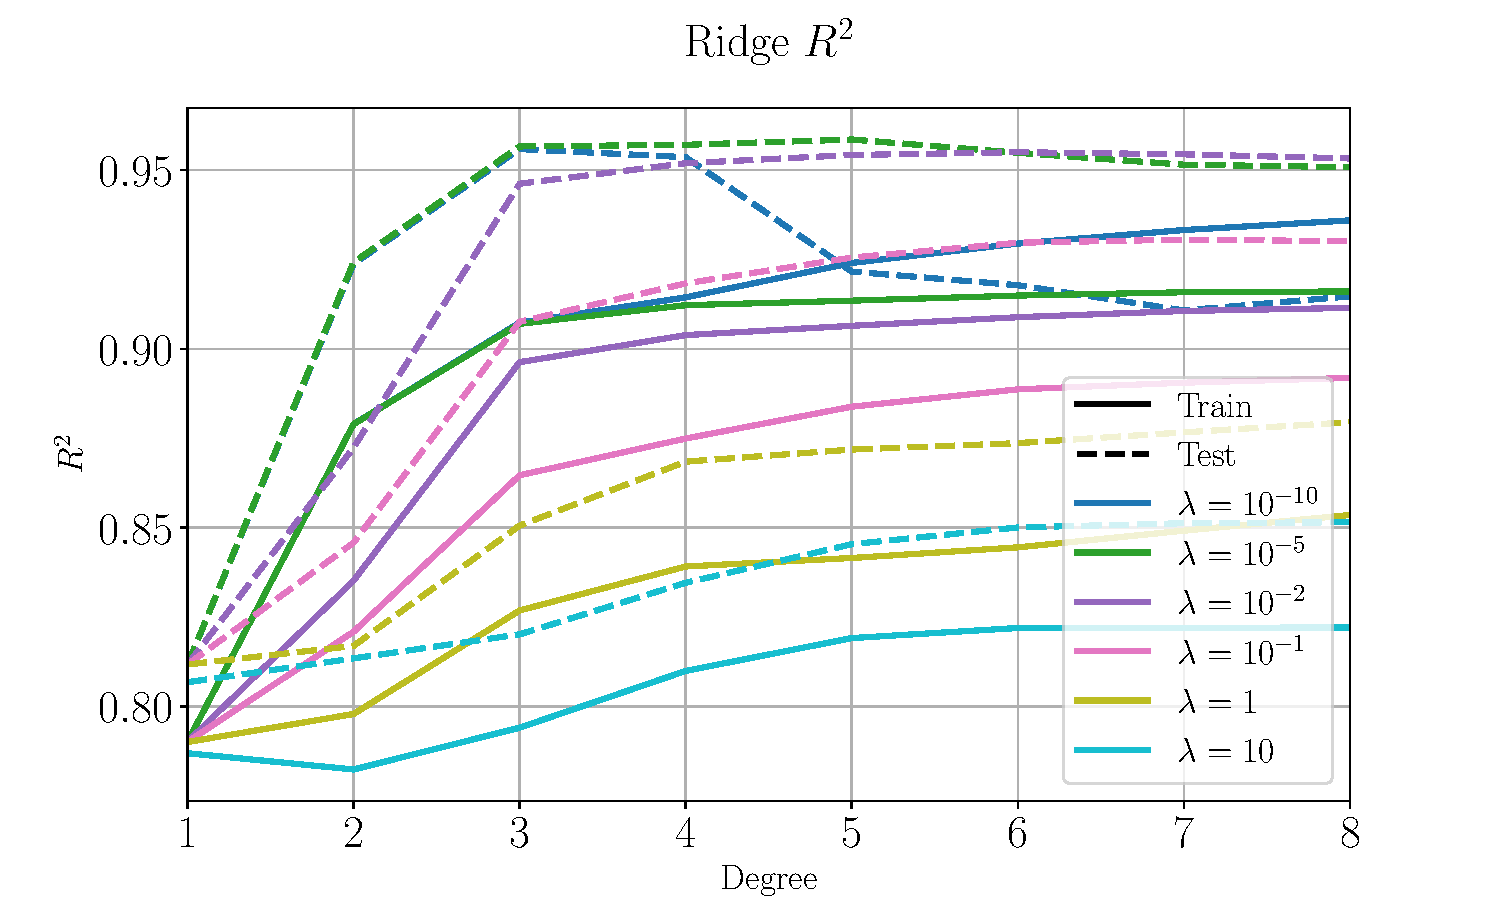
\includegraphics[width=\linewidth]{Python/Figures/Ridge-R2-degree.pdf}
	\caption{Caption}
	\label{fig:ridge_r2_degree}
\end{figure}
\begin{figure}[ht!]
	\centering
	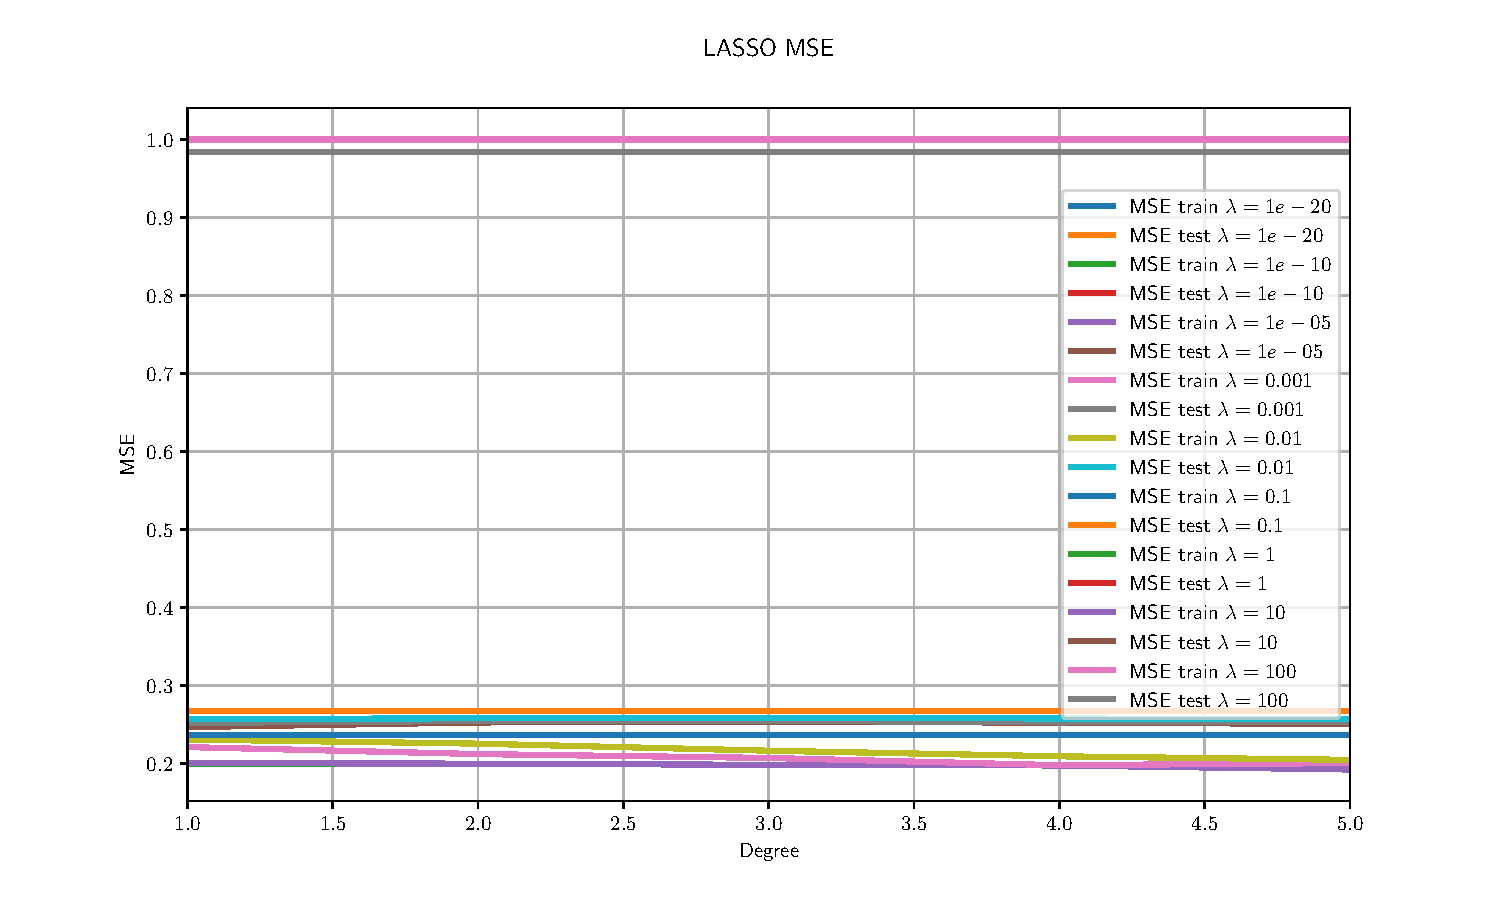
\includegraphics[width=\linewidth]{Python/Figures/LASSO-MSE-degree.pdf}
	\caption{Caption}
	\label{fig:lasso_mse_degree}
\end{figure}
\begin{figure}[ht!]
\centering
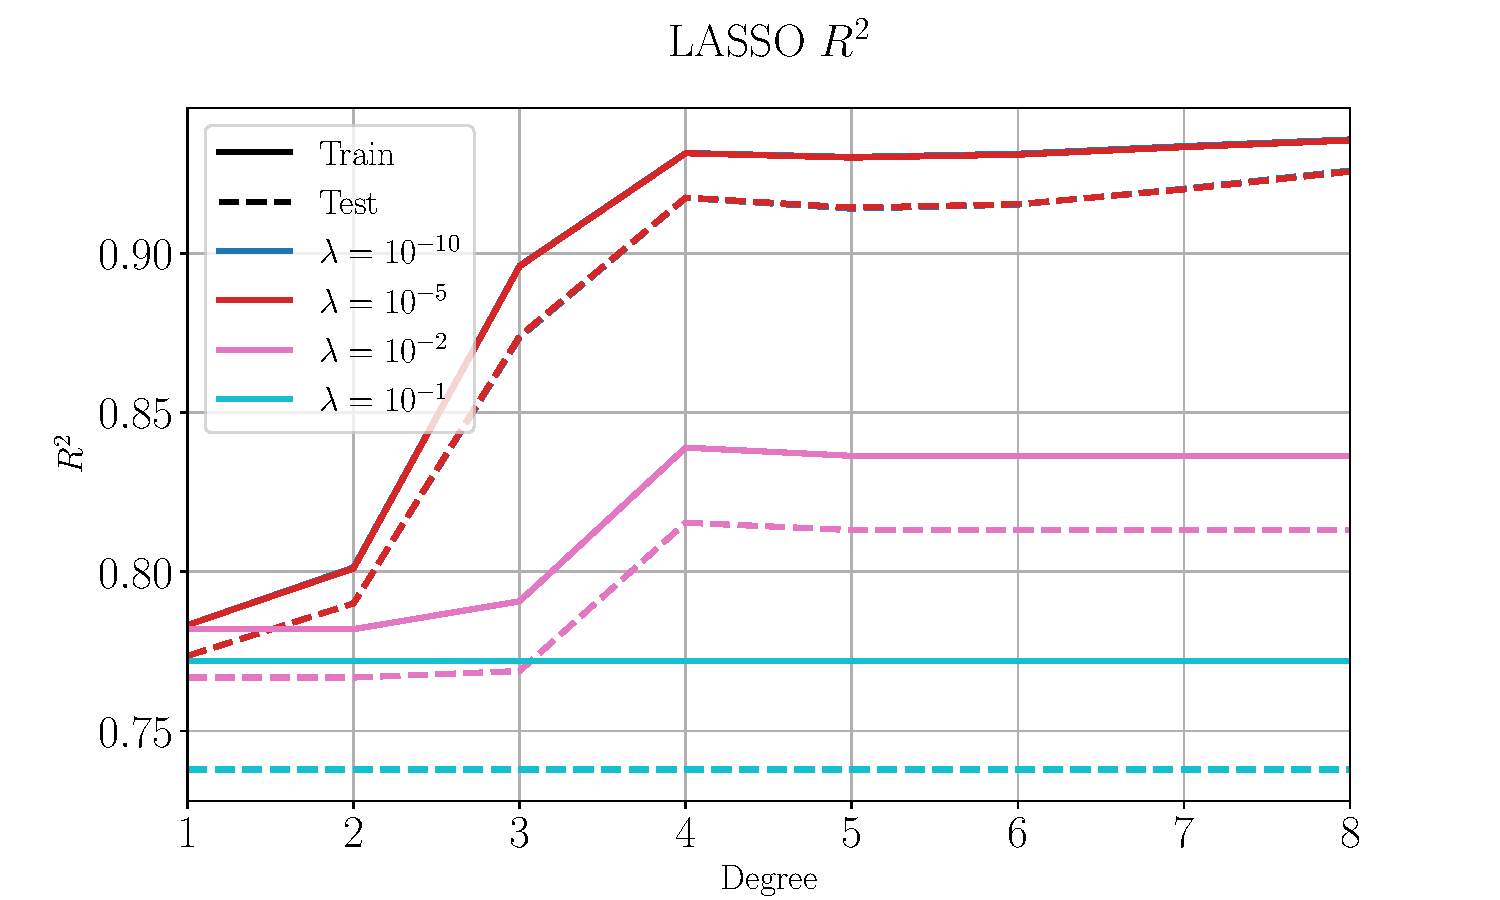
\includegraphics[width=\linewidth]{Python/Figures/LASSO-R2-degree.pdf}
\caption{Caption}
\label{fig:lasso_r2_degree}
\end{figure}

\subsection{OLS}

\subsection{Ridge}

\subsection{LASSO}

\section{Results}

\section{Discussion}

\section{Conclusion}

% Bibliography
\bibliographystyle{JHEP}
\bibliography{project1}

\appendix
\section{Derivations}
\label{Appendix:Derivations}

\subsection{Model}
The variance of $\bm y$ calculated as follows:
\begin{align*}
	\text{Var}(y_i)&=\mathbb{E}\{[y_i-\mathbb{E}(y_i)]^2\}\\
	&=\mathbb{E}\{(\bm X_{i,*}\bm\beta+\varepsilon_i)^2\}-(\bm X_{i,*}\bm\beta)^2\\
	&=(\bm X_{i,*}\bm\beta)^2+\mathbb{E}(\varepsilon_i^2)+2\mathbb{E}(\varepsilon_i)\bm X_{i,*}\bm\beta-(\bm X_{i,*}\bm\beta)^2\\
	&=\text{Var}(\varepsilon_i^2)=\sigma^2
\end{align*}
A direct way of seeing the effect of the regulator is by considering the singular value decomposition of $\bm X$. Writing $\bm X=\bm U\bm \Sigma\bm V$ where $\bm U,\bm V$ are orthogonal and $\bm \Sigma$ only contains elements on the diagonal the proof goes as follows:
\begin{align*}
	\tilde{\bm{y}}_\text{Ridge}&=\bm{X\beta}_\text{Ridge}=\bm{X}(\bm{X}^T\bm{X}+\lambda\bm I)^{-1}\bm{X}^T\bm{y}\\
	&=\bm{U\Sigma V}^T((\bm{U\Sigma V}^T)^T\bm{U\Sigma V}^T+\lambda\bm I)^{-1}(\bm{U\Sigma V}^T)^T\bm{y}\\
	&=\bm{U\Sigma V}^T(\bm{V}\bm{\Sigma}^T\bm{\Sigma}\bm{V}^T+\lambda\bm I)^{-1}\bm{V}\bm{\Sigma}^T\bm{U}^T\bm{y}\\
	&=\bm{U\Sigma V}^T(\bm{V}({\bm\Sigma}^T\bm{\Sigma}+\lambda\bm I)\bm{V}^T)^{-1}\bm{V}\bm{\Sigma}^T\bm{U}^T\bm{y}\\
	&=\bm{U\Sigma }({\bm\Sigma}^T\bm{\Sigma}+\lambda\bm I)^{-1}\bm{\Sigma}^T\bm{U}^T\bm{y}\\
	&=\sum_{j=0}^{p-1}\bm{u}_j\bm{u}_j^T\frac{\sigma_j^2}{\sigma_j^2+\lambda}\bm{y}
\end{align*}
where the last step is valid due to the orthogonality of $\bm U$ and $\sigma_j$ are the elements on the diagonal of $\bm\Sigma$.

\subsection{Coefficients}
The expectation value of the optimal parameters $\hat{\bm\beta}$ can be found to be
\begin{align*}
	\mathbb{E}(\hat{\bm\beta}_\text{OLS})&=\mathbb{E}[ (\bm X^T\bm X)^{-1}\bm X^T\bm y]\\
	&=(\bm X^T\bm X)^{-1}\bm X^T \mathbb{E}[\bm y]\\
	&=(\bm X^T\bm X)^{-1}\bm X^T\bm X\bm\beta=\bm\beta.
\end{align*}
with the variance
\begin{align*}
	\text{Var}(\hat{\bm\beta}_\text{OLS})&=\mathbb E\{ [\bm\beta-\mathbb E(\bm\beta)] [\bm\beta-\mathbb E(\bm\beta)]^T\}\\
	&=\mathbb E\{ [(\bm X^T\bm X)^{-1}\bm X^T\bm y-\bm\beta]\\
	&\quad\times[(\bm X^T\bm X)^{-1}\bm X^T\bm y-\bm\beta]^T\}\\
	&=(\bm X^T\bm X)^{-1}\bm X^T\mathbb E\{\bm y\bm y^T\}\bm X(\bm X^T\bm X)^{-1}\\
	&\quad-\bm\beta\bm\beta^T\\
	&=(\bm X^T\bm X)^{-1}\bm X^T[\bm X\bm\beta\bm\beta^T\bm X^T+\sigma^2]\bm X(\bm X^T\bm X)^{-1}\\
	&\quad-\bm\beta\bm\beta^T\\
	&=\bm\beta\bm\beta^T+\sigma^2(\bm X^T\bm X)^{-1}-\bm\beta\bm\beta^T\\
	&=\sigma^2(\bm X^T \bm X)^{-1}
\end{align*}
The optimal parameters for Ridge regressions can again be found by the same process as for OLS:
\begin{align*}
	0&=\pdv{C_\text{Ridge}}{\bm{\beta}}=-\f2n(\bm{y}-\bm{X}\bm{\beta})^T\bm{X}+2\lambda\bm{\beta}^T\\
	&=\f2n(\bm{\beta}^T\bm{X}^T\bm{X}-\bm{y}^T\bm{X})+2\lambda\bm{\beta}^T\\
	0&=\bm{\beta}^T(\bm{X}^T\bm{X}+\tilde{\lambda}\bm{I})-\bm{y}^T\bm{X}\\
	\bm{\beta}^T&=\bm{y}^T\bm{X}(\bm{X}^T\bm{X}+\tilde{\lambda}\bm{I})^{-1}\\
	\bm{\beta}&=(\bm{X}^T\bm{X}+\lambda\bm{I})^{-1}\bm{X}^T\bm{y}
\end{align*}
where we defined $\tilde{\lambda}\equiv n\lambda$, renamed $\tilde{\lambda}\to\lambda$ and used that the matrix in the parenthesis is a symmetric matrix and thus its inverse must also be symmetric. 

\subsection{Bias-Variance}
For ease of notation we write $f(\bm x)=f$ and simply ignore vector notation since everything is a scalar in the end. Then we have
\begin{align*}
	\mathbb{E}[(\bm y-\tilde{\bm y})^2]&=\mathbb{E}[(f+\bm\varepsilon-\tilde{\bm y})^2]\\
	&=\mathbb{E}[(f-\tilde{\bm y})^2]+2\underbrace{\mathbb{E}[(f-\tilde{\bm y})\bm\varepsilon]}_{=\,0}+\underbrace{\mathbb{E}[\bm\varepsilon^2]}_{=\,\sigma^2}\\
	&=\mathbb{E}[((f-\mathbb{E}[\tilde{\bm y}])-(\tilde{\bm y}-\mathbb{E}[\tilde{\bm y}]))^2]+\sigma^2\\
	&=\mathbb{E}[(f-\mathbb{E}[\tilde{\bm y}]))^2]+\mathbb{E}[(\tilde{\bm y}-\mathbb{E}[\tilde{\bm y}])^2]\\
	&-2\,\mathbb{E}[((f-\mathbb{E}[\tilde{\bm y}])(\tilde{\bm y}-\mathbb{E}[\tilde{\bm y}]))]+\sigma^2\\
	&=\text{Bias}[\tilde{\bm y}]+\text{Var}[\tilde{\bm y}]+\sigma^2\\
	&-2\,\mathbb{E}[(f-\mathbb{E}[\tilde{\bm y}])(\tilde{\bm y}-\mathbb{E}[\tilde{\bm y}])]
\end{align*}
where $\mathbb{E}[(f-\tilde{\bm y})\bm\varepsilon]=0$ is justified by $\bm\varepsilon$ being independent and we note that the wrong definition of the Bias is given in the problem text (with that definition $\sigma^2$ gets put into the `Bias'). All that remains is to show that the last term is 0. Since $\mathbb{E}[f]=f$ and $\mathbb{E}[f\,\mathbb{E}[\tilde{\bm y}]]=f\,\mathbb{E}[\mathbb{E}[\tilde{\bm y}]]=f\,\mathbb{E}[\tilde{\bm y}]$ then
\begin{align*}
	\mathbb{E}[(f-\mathbb{E}[\tilde y])(\tilde{\bm y}-\mathbb{E}[\tilde y])]&=\mathbb{E}[f\tilde{\bm y}-f\,\mathbb{E}[\tilde{\bm y}]-\tilde{\bm y}\,\mathbb{E}[\tilde y]+\mathbb{E}^2[\tilde{\bm y}]]\\
	&=f\,\mathbb{E}[\tilde{\bm y}]-f\,\mathbb{E}[\tilde{\bm y}]-\mathbb{E}^2[\tilde{\bm y}]+\mathbb{E}^2[\tilde{\bm y}]\\
	&=0
\end{align*}
which proves the claim. 

\section{}
	
\end{document}